\documentclass[conference]{IEEEtran}
\usepackage[T1]{fontenc}
\usepackage{newtxtext,newtxmath}
\usepackage{amsmath}
\usepackage{graphicx}
\usepackage{booktabs}
\usepackage{siunitx}
\usepackage[hidelinks]{hyperref}
\graphicspath{{figures/}{../data/figures/}}
\sisetup{group-minimum-digits=4}

% house style: no em dashes, so the abstract heading uses a colon
\makeatletter
\def\abstract{\normalfont\@IEEEabskeysecsize\bfseries\textit{\abstractname}:\ \relax\@IEEEgobbleleadPARNLSP}
\makeatother

\newcommand{\ugm}{\si{\micro\gram\per\cubic\metre}}
\newcommand{\col}[1]{\texttt{#1}}

% allow more floats per page so tables and figures stay near their text
\renewcommand{\topfraction}{0.85}
\renewcommand{\bottomfraction}{0.6}
\renewcommand{\textfraction}{0.1}
\renewcommand{\floatpagefraction}{0.75}
\setcounter{topnumber}{3}
\setcounter{bottomnumber}{2}
\setcounter{totalnumber}{5}

\begin{document}

\title{Six-hour PM2.5 forecasting in Beijing with gradient boosting and leak-free backtesting}

\author{\IEEEauthorblockN{Vetriselvan R, Hrishi Dongre, Pampana Sree Adithya, Ishan Goyal, Vedant Madne}
\IEEEauthorblockA{Team T024, Section A - AML/DL Project 19: Air quality forecasting via gradient boosting and LSTM models}}

\maketitle

\begin{abstract}
We forecast hourly PM2.5 at the US Embassy in Beijing one, six and 24 hours ahead, with six hours as the headline horizon, using only information available when the forecast is made. A model sees 52 inputs in six groups: PM2.5 history, rolling statistics, the calendar of the target hour, weather from the hour before the forecast, derived weather, and physics features for stagnation, southerly transport and humid build-up taken from the Beijing episode and air stagnation literature. XGBoost is tuned by random search, averaged over five seeds and blended with ridge regression. Every tuned setting is chosen on three expanding-window validation years (2011 to 2013) with a 24-hour embargo, and the 2014 test year is scored once. At six hours the blend reaches an RMSE of 51.96~\ugm, MAE 33.93 and $R^2$ 0.690 on 2014, against 61.22, 38.67 and 0.569 for persistence: 15.1\% lower RMSE, close to the 14.4\% measured during validation. Added after PM2.5 history and the calendar, weather gives the largest gain, and a raw target beats log1p, which biases forecasts low by 12.6~\ugm. Errors concentrate in high-pollution hours: hours above 150~\ugm{} are 21.2\% of validation hours but carry 50.6\% of the squared error. A mixture of experts with a learned gate for hours above 150~\ugm{} lowers validation MAE by 1.1 to 1.3\% in every seed set, but its RMSE gain is within seed noise; with the true label as gate the same experts would cut validation RMSE by 30\%, which locates the remaining limit in predicting when episodes start and end.
\end{abstract}

\section{Introduction}
Beijing's PM2.5 alternates between clean air and severe multi-day episodes driven by emissions and weather \cite{liang2015}. Forecasting it a few hours ahead supports health warnings, but a forecast is only useful if it beats the simplest rule, that PM2.5 stays at its current value (persistence), and if its accuracy is measured on data the model has never influenced \cite{tashman2000,kaufman2012}.

This project compares gradient boosting (Phase 1, this report) with recurrent and convolutional networks (Phase 2) on the UCI Beijing PM2.5 dataset \cite{uci}. A companion report \cite{datareport} covers the exploratory data analysis (EDA) and preprocessing; Section~\ref{sec:data} summarises the findings that shape the models. We chose six hours as the headline horizon before training any model: on the observed hours of 2010 to 2013, copying the current value is wrong by only 13.1~\ugm{} on average one hour ahead, while 24 hours ahead it is wrong by 69.8 and the autocorrelation has fallen to 0.33 \cite{datareport}.

Our contributions are:
\begin{itemize}
\item a direct forecasting setup with explicit look-ahead rules, an embargo between training and evaluation, and a test year guarded so that it can be scored only once (Section~\ref{sec:protocol});
\item physics-informed features from the Beijing episode literature and a five-seed ablation of every feature group and target form (Sections~\ref{sec:features} and \ref{sec:ablation});
\item a tuned XGBoost and ridge blend that beats persistence by 15.1\% RMSE at six hours on the unseen year 2014 (Section~\ref{sec:results});
\item an error analysis by season and pollution episode, and a mixture-of-experts extension that shows where the remaining error comes from (Sections~\ref{sec:errors} and \ref{sec:moe}).
\end{itemize}

\section{Related work}
\label{sec:related}

\subsection{PM2.5 meteorology in Beijing}
Liang et al. \cite{liang2015} introduced the dataset used here and showed that weather explains much of the variation in Beijing's PM2.5. Zhong et al. \cite{zhong2018} split winter episodes into a transport stage, when pollution arrives on southerly winds, and a cumulative stage under weak southerly or calm winds, a shallow boundary layer and relative humidity above 80\%, and attribute over 70\% of the cumulative explosive growth to meteorological feedback. Huang et al. \cite{huang2018} review the air stagnation index of the US National Climatic Data Center, which calls a day stagnant when the 10~m wind is below 3.2~m/s, the 500~hPa wind below 13~m/s and no precipitation falls; they find it not well suited to China and propose a boundary-layer index instead. Our physics features come from Zhong et al. and from the surface part of the older index.

\subsection{Forecasting models}
Persistence and seasonal-naive forecasts are the standard reference points for short-horizon forecasting \cite{hyndman2021}. Gradient-boosted trees \cite{chen2016} handle nonlinear interactions, missing inputs and mixed feature scales without preprocessing, which makes them a strong tabular baseline. Recurrent networks such as the LSTM \cite{hochreiter1997} read raw input windows instead of hand-built lags and are the Phase 2 candidates. Wang and Du \cite{wang2026} compare persistence, seasonal-naive, ridge, elastic net and five-seed XGBoost on 12 Beijing stations (2013 to 2017) with co-pollutants (PM10, SO\textsubscript{2}, NO\textsubscript{2}, CO, O\textsubscript{3}) and station indicators as extra inputs. Their best $R^2$ is 0.953, 0.660 and 0.242 at 1, 6 and 24 hours, with XGBoost best at six hours; we use their results as an external reference for the shape of the problem.

\subsection{Multi-step strategy}
A forecast $h$ steps ahead can come from one model applied recursively, from one model per horizon (direct), or from one model with several outputs \cite{bentaieb2012}. The recursive strategy feeds forecasts back as inputs and accumulates their errors; we use the direct strategy, one model per horizon.

\subsection{Evaluation and leakage}
Out-of-sample tests on data after the training period are the standard check of forecast accuracy \cite{tashman2000}; Bergmeir and Ben\'{i}tez \cite{bergmeir2012} show that blocked cross-validation can also work, but we keep forward-only folds. Leakage, the use of information a model would not legitimately have when it predicts, inflates scores \cite{kaufman2012}; information from the evaluation period reaching training is one form of it. Overlapping labels are removed with a gap between training and evaluation, which L\'{o}pez de Prado calls purging \cite{lopezdeprado2018}.

\subsection{Combination and experts}
Combining forecasts with weights chosen to minimise squared error often beats the individual forecasts \cite{bates1969}. A mixture of experts \cite{jacobs1991} goes further and lets a gating model weight each expert per input. When a model is trained on log1p of the target, the naive back-transform underestimates the mean; Duan's smearing factor \cite{duan1983} corrects it.

\section{Data and exploratory findings}
\label{sec:data}
The dataset \cite{uci} holds hourly PM2.5 measured at the US Embassy together with weather from Beijing Capital International Airport, 2010-01-01 to 2014-12-31 (\num{43824} hours). Only PM2.5 has missing values (\num{2067} hours, 4.72\%); the cumulative wind column is decoded into hourly speed, and the missing target is never filled \cite{datareport}. The years 2010 to 2013 are used for development; 2014 is the test year. Table~\ref{tab:eda} lists the EDA findings, all measured on 2010 to 2013, that shaped the models.

\begin{table}[!htb]
\centering
\caption{EDA findings on 2010 to 2013 and the design choices they led to \cite{datareport}}
\label{tab:eda}
\begin{tabular}{@{}p{0.5\columnwidth}p{0.42\columnwidth}@{}}
\toprule
Finding & Design choice \\
\midrule
Persistence MAE 13.1, 40.8, 69.8 at 1, 6, 24 h; autocorrelation of log1p(pm25) 0.96, 0.74, 0.33 & Six-hour headline; lags 1, 2, 3, 6, 12, 24, 48 h; rolling statistics \\
Opposite daily cycles: winter median peaks at 21:00, summer at 08:00 & Hour and month of the target hour as sine and cosine \\
North-west wind cleanest (median 31), calm and variable (cv) and south-east dirtiest (100, 93) & Wind direction, speed and NW wind run \\
First three hours of a NW spell: median change $-12.2\%$ in six hours & Hours since the wind direction changed \\
Pressure rise above 2 hPa in 3 h: median change $-21.4\%$ & Pressure tendency over 3 and 24 h \\
Relative humidity has the strongest same-hour rank correlation (Spearman 0.54); at $t+6$ wind speed leads ($-0.46$ against 0.39) & Relative humidity, humid hours \\
322 episodes of at least 6 consecutive hours above 150: slow build (median at least 55 h, 72 h look-back), fast clearing (median 14 h to a quarter of the peak, 277 episodes that clear within 72 h) & Physics features; scores on hours above 150 \\
Lunar New Year peaks 7 to 14 times the usual level & Lunar New Year flag \\
pm25 skew 1.81 & Raw and log1p targets compared \\
\bottomrule
\end{tabular}
\end{table}

\begin{figure}[!t]
\centering
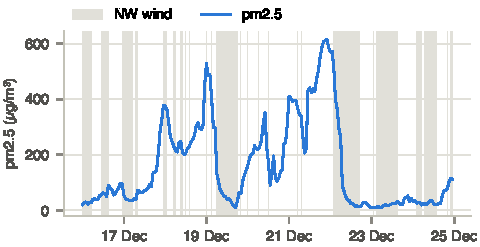
\includegraphics[width=\columnwidth]{episode.pdf}
\caption{Two episodes in December 2010: slow build-up, then collapse within hours of a sustained north-west wind spell (north-west hours shaded) \cite{datareport}.}
\label{fig:episode}
\end{figure}

\section{Problem formulation and evaluation protocol}
\label{sec:protocol}

\subsection{Direct forecasting}
Let $y_t$ be PM2.5 at hour $t$, the forecast origin. For each horizon $h \in \{1, 6, 24\}$ a separate model predicts
\begin{equation}
\hat{y}_{t+h} = f_h(\mathbf{x}_t),
\end{equation}
where $\mathbf{x}_t$ contains PM2.5 up to hour $t$, weather up to hour $t-1$, and the calendar of the target hour $t+h$, which is known in advance. Weather is taken one hour before the origin because another UCI release of the same station \cite{fivecities} has identical temperature, dew point, pressure and wind but PM2.5 shifted by one hour, and we cannot tell which clock is right; with a one-hour lag no weather input can share an hour with the target either way.

\subsection{Folds and embargo}
Fold $k$ evaluates on calendar year $Y_k$ and trains on all hours before 1 January of $Y_k$ minus a 24-hour embargo, so no training target falls in the evaluation year for any $h \le 24$ (purging in the sense of \cite{lopezdeprado2018}). The validation folds cv1, cv2 and cv3 evaluate 2011, 2012 and 2013 with one, two and three training years; the test fold trains on 2010 to 2013 and evaluates 2014. An evaluation hour is kept only if the origin and the target both lie inside the evaluation year, the target was observed, and both baselines can be computed. Every model is therefore scored on the same hours: \num{24417} pooled validation hours at six hours.

\subsection{Metrics and selection}
With errors $e_i = \hat{y}_i - y_i$ over $n$ hours,
\begin{gather}
\text{MAE} = \frac{1}{n}\sum_i |e_i|, \qquad \text{RMSE} = \sqrt{\frac{1}{n}\sum_i e_i^2}, \\
R^2 = 1 - \frac{\sum_i e_i^2}{\sum_i (y_i - \bar{y})^2}, \qquad \text{skill} = 1 - \frac{\text{RMSE}}{\text{RMSE}_{\text{persistence}}},
\end{gather}
with MAE, RMSE and the bias $\bar{e}$ in \ugm{} on the original scale and $R^2$ and skill unitless. Every tuned choice (hyperparameters, target form, ridge penalty, blend weights) minimises RMSE pooled over cv1 to cv3; fixed settings such as the fill limit, weather lag, embargo, lags and physics thresholds come from the EDA on 2010 to 2013 and the literature. Both models train on squared error, which RMSE measures, and on a fixed set of hours RMSE and $R^2$ rank models identically. Because choices are made and scored on the same folds, validation scores are slightly optimistic; the test year is the honest estimate.

\subsection{Score-once test year}
All settings were frozen before 2014 was scored, once, on 2026-10-19. The scoring step refuses to run if test scores already exist and stores a SHA-256 fingerprint of the Phase 1 configuration and the chosen settings, so a second look at the test year cannot happen silently.

\section{Features}
\label{sec:features}
Table~\ref{tab:features} lists the 52 inputs at six hours. Two parts depend on the fold or horizon and are added per fold: the calendar of the target hour, and \col{pm\_anom}, PM2.5 now minus the mean PM2.5 for that hour of day in the fold's training years. Relative humidity uses the Magnus formula \cite{alduchov1996}.

\begin{table}[!htb]
\centering
\caption{Feature groups (52 columns at $h = 6$)}
\label{tab:features}
\begin{tabular}{@{}lrp{0.62\columnwidth}@{}}
\toprule
Group & $n$ & Columns \\
\midrule
Lags & 10 & PM2.5 now and 1, 2, 3, 6, 12, 24, 48 h ago; missing flag now; missing hours in the last 24 h \\
Rolling & 15 & mean, std, max over 3, 6, 12, 24 h; change over 1 and 3 h; \col{pm\_anom} \\
Calendar & 7 & target hour and month as sin and cos, day of week, weekend, Lunar New Year eve and day \\
Weather & 11 & dew point, temperature, pressure, wind speed, cumulative wind, rain, snow, four wind directions; hour $t-1$ \\
Derived & 5 & relative humidity, pressure change over 3 and 24 h, hours since the wind direction changed, NW wind run over 24 h \\
Physics & 4 & stagnant hours in 24 h, current stagnant run, SE wind run over 24 h, humid hours in 24 h \\
\bottomrule
\end{tabular}
\end{table}

The physics group turns the episode literature into hourly inputs. An hour is stagnant when the wind is weak and no rain falls,
\begin{equation}
s_t = \mathbf{1}[\,ws_t < 3.2\ \text{m/s} \wedge \text{rain}_t = 0\,],
\end{equation}
the surface part of the stagnation index reviewed in \cite{huang2018}, applied per hour with rain as the precipitation test. From it, \col{stag24} $= \sum_{k=1}^{24} s_{t-k}$ counts stagnant hours and \col{stag\_run} is the length of the current stagnant run. \col{se\_ws24} sums south-east wind speed over 24 hours, our proxy for the southerly transport stage of \cite{zhong2018} since the data have no south-west direction, and \col{humid24} counts hours with relative humidity above 80\% (the cumulative stage). Trees split on single values and cannot build counts or run lengths themselves, so these columns add memory the weather group lacks.

Every feature at origin $t$ uses rows up to $t$ only, with one exception inside training: \col{pm\_anom} on training rows subtracts an hour-of-day mean over the whole training span. Evaluation rows use training labels only. A test cuts the data at two origins and checks that the 44 history, weather, derived and physics columns up to each cut are unchanged; further tests check that weather inputs lag the origin, that training targets respect the embargo, that adding later years never changes a fold, and that the hour-of-day climatology ignores evaluation labels.

\section{Models}
\label{sec:models}

\subsection{Baselines}
Persistence forecasts $\hat{y}_{t+h} = y_t$ and seasonal-naive forecasts $\hat{y}_{t+h} = y_{t+h-24}$, the same hour one day earlier. Both use the causal input copy of PM2.5, carried forward for at most three hours across gaps \cite{datareport}.

\subsection{Ridge regression}
Ridge regression \cite{hoerl1970} minimises $\lVert \mathbf{y} - X\boldsymbol{\beta}\rVert^2 + \alpha \lVert\boldsymbol{\beta}\rVert^2$. The penalty stabilises coefficients when inputs are collinear, as dew point, temperature and pressure are ($|r|$ 0.78 to 0.83 \cite{datareport}). PM2.5 level columns are log-transformed, missing values are filled with training medians and all columns are standardised, all fitted on training rows. The penalty $\alpha \in \{0.1, 1, 10, 100, 1000\}$ and the target (raw or log1p) are chosen together; the raw target with $\alpha = 10$ wins at one and six hours, $\alpha = 1000$ at 24 hours.

\subsection{XGBoost}
XGBoost \cite{chen2016} builds an additive model of $M$ regression trees, $\hat{y} = b + \eta\sum_{m=1}^{M} f_m(\mathbf{x})$ with base score $b$ and learning rate $\eta$, and adds trees one at a time to minimise
\begin{equation}
\mathcal{L} = \sum_i \ell(y_i, \hat{y}_i) + \sum_m \Omega(f_m), \qquad \Omega(f) = \gamma T + \tfrac{1}{2}\lambda \lVert \mathbf{w}\rVert^2,
\end{equation}
where $T$ is the number of leaves and $\mathbf{w}$ the leaf values. With a second-order expansion of the loss, $g_i$ and $h_i$ its first and second derivatives at the current prediction, and $G_j$, $H_j$ their sums over the rows in leaf $j$, the best leaf value and the gain of a split into left and right children are
\begin{gather}
w_j^{*} = -\frac{G_j}{H_j + \lambda}, \\
\text{gain} = \frac{1}{2}\left[\frac{G_L^2}{H_L+\lambda} + \frac{G_R^2}{H_R+\lambda} - \frac{(G_L+G_R)^2}{H_L+H_R+\lambda}\right] - \gamma.
\end{gather}
For XGBoost's squared-error objective $\frac{1}{2}(\hat{y}-y)^2$, $h_i = 1$, so $H_j$ counts rows and \col{min\_child\_weight} sets the minimum leaf size. We leave $\gamma$ at its default of 0, so only the $\lambda$ penalty acts.

Training uses learning rate 0.05 and up to \num{2000} trees. Early stopping (100 rounds) watches the last 90 days of the training span, with an $h$-hour gap before them so no fitting target falls inside, and the model is then refitted on the whole span with the chosen number of trees. A random search draws 20 candidates from depth $\{3,4,5,6,8\}$, \col{min\_child\_weight} $\{1,5,10,20\}$, row subsample $\{0.6,0.8,1.0\}$, column subsample $\{0.5,0.7,0.9\}$ and $\lambda \in \{0.1,1,10\}$. At six hours the search chose depth 4, \col{min\_child\_weight} 20, row subsample 1.0, column subsample 0.5 and $\lambda = 1$, with 127 trees on average over the folds.

\subsection{Target forms}
Each candidate is tried with two target forms: the level $y_{t+h}$, and the change $y_{t+h} - y_t$, added back to the current value. A tree predicts averages of training targets, so a level model cannot go far beyond the largest value it has seen, while a change model starts from the current value. The change form won at one hour (RMSE 22.54 against 23.81) and 24 hours (83.30 against 83.48), the level form at six hours (56.84 against 57.18). We also compare training on $z = \log(1+y)$: since $\mathbb{E}[\exp z] \ge \exp \mathbb{E}[z]$, undoing the log underestimates the mean, which Duan's smearing factor $s = \frac{1}{n}\sum_i \exp(z_i - \hat{z}_i)$ \cite{duan1983}, computed on the early-stopping period, corrects as $\hat{y} = s\exp(\hat{z}) - 1$.

\subsection{Ensembles}
The seed ensemble averages five XGBoost models that differ only in their random seed, which reduces the variance from row and column subsampling. A spike expert uses the same settings with the quantile loss $\rho_q(u) = u\,(q - \mathbf{1}[u < 0])$ with $u = y - \hat{y}$ at $q = 0.9$, so it aims high on purpose. The blend
\begin{equation}
\hat{y} = a\,\hat{y}_{\text{xgb}} + b\,\hat{y}_{\text{spike}} + c\,\hat{y}_{\text{ridge}}, \quad a, b, c \ge 0,\ a+b+c = 1,
\end{equation}
takes its weights from a 0.1 grid by pooled RMSE \cite{bates1969}. It chose $(a, b, c) = (0.7, 0, 0.3)$, $(0.6, 0, 0.4)$ and $(0.3, 0, 0.7)$ at 1, 6 and 24 hours; the spike expert never received weight.

\section{Results}
\label{sec:results}
Table~\ref{tab:results} shows validation and test scores. On both, the blend has the lowest RMSE at every horizon, and XGBoost has a slightly lower MAE at one hour and, on the test year, at six hours. Seasonal-naive is the weakest forecast except at 24 hours, where it equals persistence.

\begin{table*}[!t]
\centering
\caption{Scores by horizon. Validation: pooled over 2011 to 2013, used for every choice. Test: 2014, scored once. RMSE and MAE in \ugm.}
\label{tab:results}
\begin{tabular}{@{}lrrrrrrrrr@{}}
\toprule
 & \multicolumn{3}{c}{$h = 1$} & \multicolumn{3}{c}{$h = 6$} & \multicolumn{3}{c}{$h = 24$} \\
\cmidrule(lr){2-4}\cmidrule(lr){5-7}\cmidrule(l){8-10}
Model & RMSE & MAE & $R^2$ & RMSE & MAE & $R^2$ & RMSE & MAE & $R^2$ \\
\midrule
\multicolumn{10}{@{}l}{\textit{Validation, 2011 to 2013}} \\
Persistence & 24.02 & 12.82 & 0.931 & 65.77 & 40.23 & 0.483 & 101.33 & 69.34 & $-$0.229 \\
Seasonal-naive & 101.36 & 69.41 & $-$0.229 & 101.42 & 69.42 & $-$0.230 & 101.33 & 69.34 & $-$0.229 \\
Ridge & 23.07 & 13.15 & 0.936 & 57.66 & 38.27 & 0.602 & 82.21 & 60.30 & 0.191 \\
XGBoost (5 seeds) & 22.53 & \textbf{12.21} & 0.939 & 56.81 & 36.46 & 0.614 & 83.63 & 60.56 & 0.163 \\
Spike expert ($q=0.9$) & 30.68 & 20.85 & 0.887 & 82.70 & 62.21 & 0.182 & 136.54 & 109.23 & $-$1.231 \\
Blend & \textbf{22.45} & 12.23 & \textbf{0.940} & \textbf{56.33} & \textbf{36.41} & \textbf{0.621} & \textbf{81.97} & \textbf{59.93} & \textbf{0.196} \\
\midrule
\multicolumn{10}{@{}l}{\textit{Test, 2014}} \\
Persistence & 21.98 & 11.92 & 0.945 & 61.22 & 38.67 & 0.569 & 99.02 & 67.49 & $-$0.121 \\
Seasonal-naive & 98.87 & 67.36 & $-$0.121 & 98.74 & 67.30 & $-$0.121 & 99.02 & 67.49 & $-$0.121 \\
Ridge & 21.41 & 12.01 & 0.947 & 54.20 & 36.11 & 0.662 & 81.63 & 60.13 & 0.238 \\
XGBoost (5 seeds) & 20.74 & \textbf{11.27} & 0.951 & 52.21 & \textbf{33.79} & 0.687 & 83.08 & 60.23 & 0.211 \\
Spike expert ($q=0.9$) & 28.90 & 19.43 & 0.904 & 76.09 & 56.28 & 0.334 & 131.73 & 105.25 & $-$0.984 \\
Blend & \textbf{20.64} & 11.30 & \textbf{0.951} & \textbf{51.96} & 33.93 & \textbf{0.690} & \textbf{81.49} & \textbf{59.78} & \textbf{0.241} \\
\bottomrule
\end{tabular}
\end{table*}

\subsection{Generalisation to 2014}
2014 is an easier year than the validation years: persistence alone explains 56.9\% of the six-hour variance against 48.3\%. Absolute errors are therefore lower, and the fair comparison is skill. The blend's six-hour RMSE skill is 15.1\% on 2014 against 14.4\% on validation (MAE skill 12.3\% against 9.5\%), so the gain carried over to unseen data. Our $R^2$ of 0.951, 0.690 and 0.241 at 1, 6 and 24 hours is close to the 0.953, 0.660 and 0.242 reported for 12 stations with co-pollutant inputs \cite{wang2026}; the data differ, so this compares the shape of the problem, not the models.

\subsection{Choice of horizon}
Fig.~\ref{fig:horizon} sweeps the horizon with one XGBoost seed; horizons 3 and 12 reuse the six-hour settings, while 1, 6 and 24 use their own. Skill keeps rising with $h$ because persistence degrades faster than the model, so skill alone does not pick a horizon. $R^2$ completes the argument: at one hour persistence already explains 93\% of the variance, and beyond six hours XGBoost explains less than half (0.365 at 12 hours). Six hours is the longest tested horizon at which the model explains most of the variance (0.614) while clearly beating persistence (13.6\% RMSE skill). The headline was fixed from the EDA before training; this sweep confirms it.

\begin{figure}[!t]
\centering
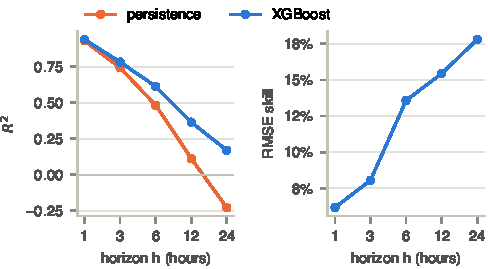
\includegraphics[width=\columnwidth]{horizon.pdf}
\caption{Validation $R^2$ of persistence and XGBoost (left) and XGBoost RMSE skill over persistence (right) by horizon, XGBoost with one seed. Horizons 3 and 12 reuse the six-hour settings.}
\label{fig:horizon}
\end{figure}

\subsection{Ablation}
\label{sec:ablation}
Fig.~\ref{fig:ablation} adds feature groups one at a time at six hours; each point is the mean forecast of five seeds, because two single fits on the same 52 columns in a different order differed by 0.74 RMSE. Added after PM2.5 history, rolling statistics and the calendar, weather brings the largest gain (60.16 to 58.02); derived weather and the physics group add 0.85 and 0.36 more. A group's gain depends on the order in which it is added. Table~\ref{tab:target} compares target forms with all features. Training on log1p biases forecasts low by 12.6~\ugm, as the inequality above predicts; smearing overcorrects to $+7.1$, and the raw level is best on RMSE.

\begin{figure}[!t]
\centering
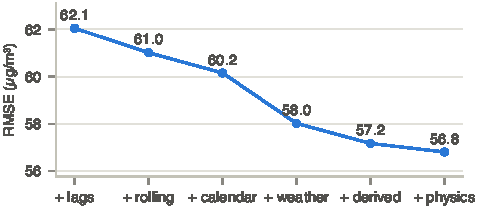
\includegraphics[width=\columnwidth]{ablation.pdf}
\caption{Validation RMSE at six hours as feature groups are added (XGBoost, mean of 5 seeds).}
\label{fig:ablation}
\end{figure}

\begin{table}[!htb]
\centering
\caption{Target form at six hours (XGBoost, 5 seeds, validation)}
\label{tab:target}
\begin{tabular}{@{}lrrrr@{}}
\toprule
Target & RMSE & MAE & $R^2$ & Bias \\
\midrule
Level, log1p & 59.96 & 37.03 & 0.570 & $-$12.63 \\
Level, log1p + smearing & 58.11 & 37.19 & 0.596 & 7.10 \\
Level, raw & \textbf{56.81} & 36.46 & \textbf{0.614} & 1.71 \\
Change, raw & 58.05 & \textbf{36.42} & 0.597 & 0.89 \\
\bottomrule
\end{tabular}
\end{table}

\subsection{Feature importance}
Table~\ref{tab:importance} ranks inputs by permutation importance \cite{breiman2001}: the rise in validation RMSE when one column is shuffled, for one seed fitted on cv3 and measured on 2013. \col{pm\_anom} dominates; it carries the current level and how unusual it is for that hour, so it overlaps with \col{pm\_0}. Two of the four physics features rank third and sixth, ahead of every raw weather column, and the three-hour pressure tendency and south-east wind follow.

\begin{table}[!htb]
\centering
\caption{Top 10 features at six hours (cv3, one seed, evaluated on 2013)}
\label{tab:importance}
\begin{tabular}{@{}llrr@{}}
\toprule
Feature & Group & Permutation (\ugm) & Gain share \\
\midrule
\col{pm\_anom} & rolling & 19.32 & 28.4\% \\
\col{pm\_0} & lags & 2.35 & 9.2\% \\
\col{stag\_run} & physics & 1.95 & 1.5\% \\
\col{hour\_cos} & calendar & 1.65 & 2.0\% \\
\col{pm\_mean24} & rolling & 1.49 & 2.9\% \\
\col{stag24} & physics & 1.39 & 2.4\% \\
\col{pres\_diff3} & derived & 1.11 & 1.1\% \\
\col{wd\_se} & weather & 1.04 & 1.5\% \\
\col{month\_cos} & calendar & 0.73 & 1.3\% \\
\col{ws} & weather & 0.73 & 1.1\% \\
\bottomrule
\end{tabular}
\end{table}

\subsection{Where the errors are}
\label{sec:errors}
Table~\ref{tab:breakdown} splits the six-hour validation error by season and for high-pollution hours, where PM2.5 at the target hour exceeds 150~\ugm{} (single hours, unlike the episodes of Table~\ref{tab:eda}). Winter error is 1.7 times the spring error. These hours are 21.2\% of the hours but carry 50.6\% of the blend's squared error, and the blend predicts them 55.3~\ugm{} too low on average; the top 5\% of hours alone carry 53.9\% of the squared error. The spike expert is best on these hours (RMSE 75.97) but far worse overall (82.70), which is why the blend gave it no weight. Fig.~\ref{fig:window} shows the typical failure: the blend follows the build-up but lags the sharp rises and clearings.

\begin{table}[!htb]
\centering
\caption{Six-hour validation RMSE by subset (\ugm)}
\label{tab:breakdown}
\begin{tabular}{@{}lrrrr@{}}
\toprule
Subset & Hours & Persistence & XGBoost & Blend \\
\midrule
Winter (DJF) & \num{6064} & 88.79 & 77.35 & 75.57 \\
Spring (MAM) & \num{6000} & 51.08 & 44.85 & 45.08 \\
Summer (JJA) & \num{6051} & 51.57 & 45.47 & 45.68 \\
Autumn (SON) & \num{6302} & 64.33 & 53.34 & 53.48 \\
Above 150 ($y > 150$) & \num{5169} & 89.21 & 89.39 & 87.08 \\
All & \num{24417} & 65.77 & 56.81 & 56.33 \\
\bottomrule
\end{tabular}
\end{table}

\begin{figure}[!t]
\centering
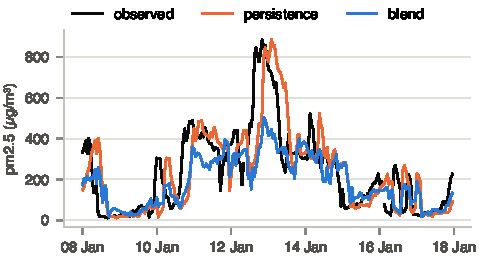
\includegraphics[width=\columnwidth]{window.pdf}
\caption{Six-hour forecasts in January 2013 (validation year of cv3), plotted at their target time.}
\label{fig:window}
\end{figure}

\subsection{Air quality categories}
To read the forecasts as warnings, we map them to the six PM2.5 categories of China's AQI regulation HJ 633-2012 \cite{hj633}, in force for these years and replaced by HJ 633-2026 in March 2026 (breakpoints 35, 75, 115, 150 and 250~\ugm). The regulation uses 24-hour means, so applying it to single hours is for illustration only, and the test year is not used because it may be scored only once. On the validation years (Table~\ref{tab:aqi}) the blend lowers the MAE from 41.4\% to 37.5\% of the mean level (97.1~\ugm) and is within one category more often, but it hits the exact category slightly less often than persistence, which is exact whenever the level does not change.

\begin{table}[!htb]
\centering
\caption{HJ 633-2012 categories at six hours, validation years (\%)}
\label{tab:aqi}
\begin{tabular}{@{}lrr@{}}
\toprule
 & Persistence & Blend \\
\midrule
MAE as share of mean level & 41.4 & \textbf{37.5} \\
Exact category & \textbf{49.0} & 47.9 \\
Within one category & 84.1 & \textbf{87.3} \\
Correct above-75 call & 79.3 & \textbf{80.4} \\
Correct above-150 call & 86.1 & \textbf{87.7} \\
\bottomrule
\end{tabular}
\end{table}

\section{Extension: mixture of experts}
\label{sec:moe}
The quantile spike expert received no weight in the blend; a likely reason is that a fixed weight lifts every hour. A mixture of experts \cite{jacobs1991} lets a gate weight an expert hour by hour. We built one with a new spike expert at six hours on the validation years only; 2014 is not used.

\subsection{Design}
The normal expert is the frozen blend. The spike expert is XGBoost with squared error trained only on hours whose target exceeds 150~\ugm{} (\num{1952}, \num{3735} and \num{5358} training hours in cv1 to cv3). A gate, an XGBoost classifier with the same inputs and settings, estimates $p = P(y_{t+6} > 150 \mid \mathbf{x}_t)$. Two combinations are compared:
\begin{gather}
\hat{y}_{\text{gate}} = \hat{y}_{\text{normal}} + \lambda\,p\,(\hat{y}_{\text{spike}} - \hat{y}_{\text{normal}}), \\
\hat{y}_{\text{split}} = (1-p)\,\hat{y}_{\text{quiet}} + p\,\hat{y}_{\text{spike}},
\end{gather}
with $\lambda$ chosen on a 0.1 grid (0.1) and a quiet expert trained on hours at or below 150. If $p$ equals the true probability $P(y_{t+6} > 150 \mid \mathbf{x}_t)$ and each expert estimates its group's conditional mean given $\mathbf{x}_t$, $\hat{y}_{\text{split}}$ is the conditional mean $\mathbb{E}[y_{t+6} \mid \mathbf{x}_t]$ by the law of total expectation, the quantity RMSE rewards.

\subsection{Gate quality}
The gate separates hours above 150 well (Table~\ref{tab:gate}) and beats the current level alone everywhere, most of all where it matters: onsets (target above 150, origin at most 150) and clearings (origin above 150, target at most 150). It is calibrated within 0.033 in every probability band (Fig.~\ref{fig:calibration}). Among hours that start above 150, telling clearings from hours that stay high is the hardest case, with an AUC of only 0.734.

\begin{table}[!htb]
\centering
\caption{Gate quality, validation years}
\label{tab:gate}
\begin{tabular}{@{}lrr@{}}
\toprule
 & Gate $p$ & PM2.5 now alone \\
\midrule
AUC, all hours & 0.923 & 0.904 \\
AUC, origin at most 150 (\num{1688} onsets) & 0.883 & 0.846 \\
AUC, origin above 150 (\num{1697} clearings) & 0.734 & 0.645 \\
Brier score & 0.088 & \\
\bottomrule
\end{tabular}
\end{table}

\begin{figure}[!t]
\centering
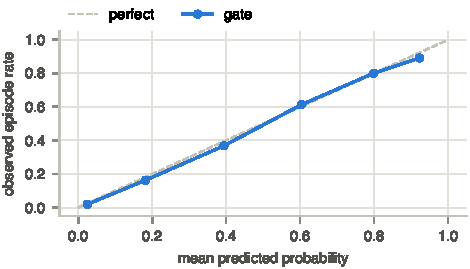
\includegraphics[width=\columnwidth]{calibration.pdf}
\caption{Gate calibration: mean predicted probability against the observed share of hours above 150 in six probability bands, validation years.}
\label{fig:calibration}
\end{figure}

\subsection{Results}
Table~\ref{tab:moe} compares the combinations. The soft split lowers MAE by 0.42~\ugm{} (1.2\%) and RMSE by 0.07. Rebuilt with three sets of five seeds, the MAE gain is 0.42, 0.42 and 0.46 while the normal expert itself moves by only 0.05 between sets, so it is real; the RMSE gain is 0.07, 0.01 and 0.20, as large as the 0.12 the normal expert itself moves, so it is not reliable. A hard switch at $p = 0.5$ is much worse on both RMSE and MAE, because every wrong call hands the hour to the wrong expert in full. With the true label as gate, the same experts reach RMSE 39.46, 30\% below the blend. This is a reference for perfect classification rather than a strict bound, but it shows that the gate limits the mixture more than the experts do.

\begin{table}[!htb]
\centering
\caption{Mixture of experts at six hours, validation years (RMSE and MAE in \ugm)}
\label{tab:moe}
\setlength{\tabcolsep}{4pt}
\begin{tabular}{@{}lrrrrr@{}}
\toprule
 & & & \multicolumn{3}{c}{RMSE on} \\
\cmidrule(l){4-6}
Model & RMSE & MAE & $y > 150$ & onset & clearing \\
\midrule
Persistence & 65.77 & 40.23 & 89.21 & 108.17 & 162.63 \\
Normal (blend) & 56.33 & 36.41 & 87.08 & 92.42 & 111.63 \\
Gate, $\lambda = 0.1$ & 56.31 & 36.40 & 85.27 & 90.95 & 114.34 \\
Split, soft & \textbf{56.26} & \textbf{35.99} & 86.57 & 92.64 & 113.20 \\
Split, hard ($p > 0.5$) & 61.24 & 38.12 & 89.83 & 108.19 & 140.14 \\
Split, true label & 39.46 & 27.29 & 64.88 & 54.93 & 42.26 \\
\bottomrule
\end{tabular}
\end{table}

\section{Discussion and limitations}
\label{sec:discussion}
The mixture result suggests why further feature or model tuning brings little. With an exact gate, a soft mixture estimates the same conditional mean as a single regression on the same inputs, so it has little to add when the gate reads the same inputs. Its weakest case is clearing (AUC 0.734); a plausible reason, not tested here, is that the north-west wind that ends an episode often arrives after the last weather input at $t-1$. Larger gains need more information, such as a longer input history, upstream stations or weather forecasts.

Validation scores are selection scores and slightly optimistic, and RMSE is a noisy selection metric here: with half of the squared error in a fifth of the hours, small differences between models are not reliable, which is why the mixture-of-experts gains are checked over three seed sets. The data come from one station without PM10, other pollutants or boundary-layer height. The one-hour weather lag guards against an unresolved clock offset between PM2.5 and weather and may cost some accuracy if the clocks agree. The air quality categories are applied to hourly values. Finally, 2014 is a single test year, and an easier one than the validation years.

\section{Conclusion and Phase 2}
A leak-free gradient boosting pipeline forecasts PM2.5 six hours ahead with 15.1\% lower RMSE than persistence on an unseen year, using PM2.5 history, weather and physics-informed stagnation features. The remaining error sits in the onset and clearing of pollution episodes, and a gate that knew the true label would cut validation RMSE by 30\% against the blend. Phase 2 will train an LSTM or temporal CNN on fixed input windows under the same folds and test protocol, and will test whether a recurrent gate that reads a longer history can supply the information the tree-based gate lacks.

\section*{Reproducibility}
The code is public at \url{https://github.com/Vetri-78640/aml_dl_pm2.5}: a Python package (\texttt{src/aqf}) for data, features, models, metrics and figures, configuration files for the data, Phase 1 and the mixture of experts, four notebooks (EDA, preprocessing, Phase 1 models, mixture of experts) and 22 automated tests covering the data pipeline, causality, the embargo and model behaviour. The Phase 1 notebook runs in about seven minutes and the mixture-of-experts notebook in under three; scores are saved as CSV files and settings, timings and the test fingerprint as JSON under \texttt{reports/}.

\section*{Team contributions}
\begin{itemize}
\item \textbf{Vetriselvan R}: Phase 1 experiments, research, physics features and the mixture of experts (gate, notebook and model history).
\item \textbf{Ishan Goyal}: exploratory data analysis on the original data and the combined data report.
\item \textbf{Vedant Madne}: preprocessing pipeline and tests, preprocessing walkthrough and feature tests.
\item \textbf{Pampana Sree Adithya}: preprocessing report and figures, skew check on the development years, calendar and humidity feature builders.
\item \textbf{Hrishi Dongre}: baselines, ridge and XGBoost models, Phase 1 experiments and results.
\end{itemize}

\begin{thebibliography}{99}
\bibitem{uci} S. Chen, ``Beijing PM2.5,'' UCI Machine Learning Repository, 2015, doi: 10.24432/C5JS49.
\bibitem{liang2015} X. Liang, T. Zou, B. Guo, S. Li, H. Zhang, S. Zhang, H. Huang, and S. X. Chen, ``Assessing Beijing's PM2.5 pollution: severity, weather impact, APEC and winter heating,'' \emph{Proc. R. Soc. A}, vol. 471, no. 2182, Art. no. 20150257, 2015.
\bibitem{datareport} Vetriselvan R, H. Dongre, P. S. Adithya, I. Goyal, and V. Madne, ``Data understanding and leak-free preprocessing for short-horizon PM2.5 forecasting in Beijing,'' Team T024 project report, 2026.
\bibitem{fivecities} S. Chen, ``PM2.5 data of five Chinese cities,'' UCI Machine Learning Repository, 2016, doi: 10.24432/C52K58.
\bibitem{zhong2018} J. Zhong, X. Zhang, Y. Dong, Y. Wang, C. Liu, J. Wang, Y. Zhang, and H. Che, ``Feedback effects of boundary-layer meteorological factors on cumulative explosive growth of PM2.5 during winter heavy pollution episodes in Beijing from 2013 to 2016,'' \emph{Atmos. Chem. Phys.}, vol. 18, pp. 247--258, 2018, doi: 10.5194/acp-18-247-2018.
\bibitem{huang2018} Q. Huang, X. Cai, J. Wang, Y. Song, and T. Zhu, ``Climatological study of the Boundary-layer air Stagnation Index for China and its relationship with air pollution,'' \emph{Atmos. Chem. Phys.}, vol. 18, pp. 7573--7593, 2018, doi: 10.5194/acp-18-7573-2018.
\bibitem{hyndman2021} R. J. Hyndman and G. Athanasopoulos, \emph{Forecasting: Principles and Practice}, 3rd ed. Melbourne, Australia: OTexts, 2021.
\bibitem{chen2016} T. Chen and C. Guestrin, ``XGBoost: A scalable tree boosting system,'' in \emph{Proc. 22nd ACM SIGKDD Int. Conf. Knowledge Discovery and Data Mining}, 2016, pp. 785--794, doi: 10.1145/2939672.2939785.
\bibitem{hochreiter1997} S. Hochreiter and J. Schmidhuber, ``Long short-term memory,'' \emph{Neural Computation}, vol. 9, no. 8, pp. 1735--1780, 1997.
\bibitem{wang2026} Y. Wang and R. Du, ``Same-hour estimation and multi-horizon forecasting of PM2.5 in Beijing: Model comparison and feature-group contributions,'' arXiv:2607.07279v3 [stat.AP], Aug. 2026.
\bibitem{bentaieb2012} S. Ben Taieb, G. Bontempi, A. F. Atiya, and A. Sorjamaa, ``A review and comparison of strategies for multi-step ahead time series forecasting based on the NN5 forecasting competition,'' \emph{Expert Systems with Applications}, vol. 39, no. 8, pp. 7067--7083, 2012.
\bibitem{tashman2000} L. J. Tashman, ``Out-of-sample tests of forecasting accuracy: an analysis and review,'' \emph{Int. J. Forecasting}, vol. 16, no. 4, pp. 437--450, 2000.
\bibitem{bergmeir2012} C. Bergmeir and J. M. Ben\'{i}tez, ``On the use of cross-validation for time series predictor evaluation,'' \emph{Information Sciences}, vol. 191, pp. 192--213, 2012.
\bibitem{kaufman2012} S. Kaufman, S. Rosset, C. Perlich, and O. Stitelman, ``Leakage in data mining: Formulation, detection, and avoidance,'' \emph{ACM Trans. Knowl. Discov. Data}, vol. 6, no. 4, Art. no. 15, 2012.
\bibitem{lopezdeprado2018} M. L\'{o}pez de Prado, \emph{Advances in Financial Machine Learning}. Hoboken, NJ, USA: Wiley, 2018.
\bibitem{bates1969} J. M. Bates and C. W. J. Granger, ``The combination of forecasts,'' \emph{Operational Research Quarterly}, vol. 20, no. 4, pp. 451--468, 1969.
\bibitem{jacobs1991} R. A. Jacobs, M. I. Jordan, S. J. Nowlan, and G. E. Hinton, ``Adaptive mixtures of local experts,'' \emph{Neural Computation}, vol. 3, no. 1, pp. 79--87, 1991.
\bibitem{duan1983} N. Duan, ``Smearing estimate: A nonparametric retransformation method,'' \emph{J. Amer. Statist. Assoc.}, vol. 78, no. 383, pp. 605--610, 1983.
\bibitem{alduchov1996} O. A. Alduchov and R. E. Eskridge, ``Improved Magnus form approximation of saturation vapor pressure,'' \emph{J. Appl. Meteorol.}, vol. 35, no. 4, pp. 601--609, 1996.
\bibitem{hoerl1970} A. E. Hoerl and R. W. Kennard, ``Ridge regression: Biased estimation for nonorthogonal problems,'' \emph{Technometrics}, vol. 12, no. 1, pp. 55--67, 1970.
\bibitem{breiman2001} L. Breiman, ``Random forests,'' \emph{Machine Learning}, vol. 45, no. 1, pp. 5--32, 2001.
\bibitem{hj633} Ministry of Environmental Protection of China, \emph{Technical Regulation on Ambient Air Quality Index (on trial)}, HJ 633-2012, 2012 (replaced by HJ 633-2026 on 1 March 2026).
\end{thebibliography}

\end{document}
